
\documentclass[12pt,a4paper, twosite]{article}
\usepackage[utf8]{inputenc}
\usepackage[T1]{fontenc}
\usepackage{graphicx}
\usepackage{grffile}
\usepackage{longtable}
\usepackage{wrapfig}
\usepackage{rotating}
\usepackage[normalem]{ulem}
\usepackage{amsmath}
\usepackage{textcomp}
\usepackage{amssymb}
\usepackage{capt-of}
\usepackage{hyperref}
\usepackage[left=2.00cm, right=2.50cm, top=2.50cm, bottom=2.00cm]{geometry}
\usepackage{fancyhdr}
\fancyhead[RO,LE]{\thepage}
\fancyhead[LO]{\emph{\uppercase{\leftmark}}}
\fancyfoot{}
\renewcommand{\headrulewidth}{1.0pt}
\pagestyle{fancy}
\date{March 22, 2024.}
\title{Manifests for PWA.}

\hypersetup{
 pdfauthor={Velazquez Gonzalez Jesus Alejandro},
 pdftitle={manifests for pwa},
 pdfkeywords={},
 pdfsubject={}
 pdfcreator={Emacs 26.2 (Org mode 9.1.9)}, 
 pdflang={English}}
\begin{document}

\maketitle

\newpage
\tableofcontents

\newpage

\section{Introduction}
\label{sec:org60390fa}

In this document we will talk about fot the manifests and how can use it in a pwa.

\subsection{Purpose}
\label{sec:org434c3ef}

The purpose of this document is to provide a detailed description of the manifests and how can use it to develop a pwa application.

\subsection{References}
\label{sec:org62711e0}

\begin{thebibliography}
{9}

\bibitem{Caching - Progressive web apps} MDN (2023, June 28) MDN Web Docs.  \url{https://developer.mozilla.org/en-US/docs/Web/Manifest}



\end{thebibliography}


\section{Manifests}
\label{sec:orgc1c4017}
Manifests is a JSON (JavaScript Object Notation) file that provides metadata about a Progressive Web App (PWA). This metadata includes information such as the app's name, icons, colors, display modes, and other properties that influence how the app appears and behaves when installed on a user's device.



\subsection{Deploying a manifest}

To deploy a manifest, you need to create a file named manifest.json in the root directory of your web app. The manifest.json file must be served with the correct MIME type, application/manifest+json, and linked to from your web app using a link element in the head of your HTML document.


\subsection{Splash screens}

In some browsers and operating systems, a splash screen is displayed when an installed PWA is launched. This splash screen is automatically generated and its appearance is defined by members in the web app manifest, specifically:

\subsection{Manifests example}
\label{sec:org2498090}

\begin{figure}
  \begin{centering}
  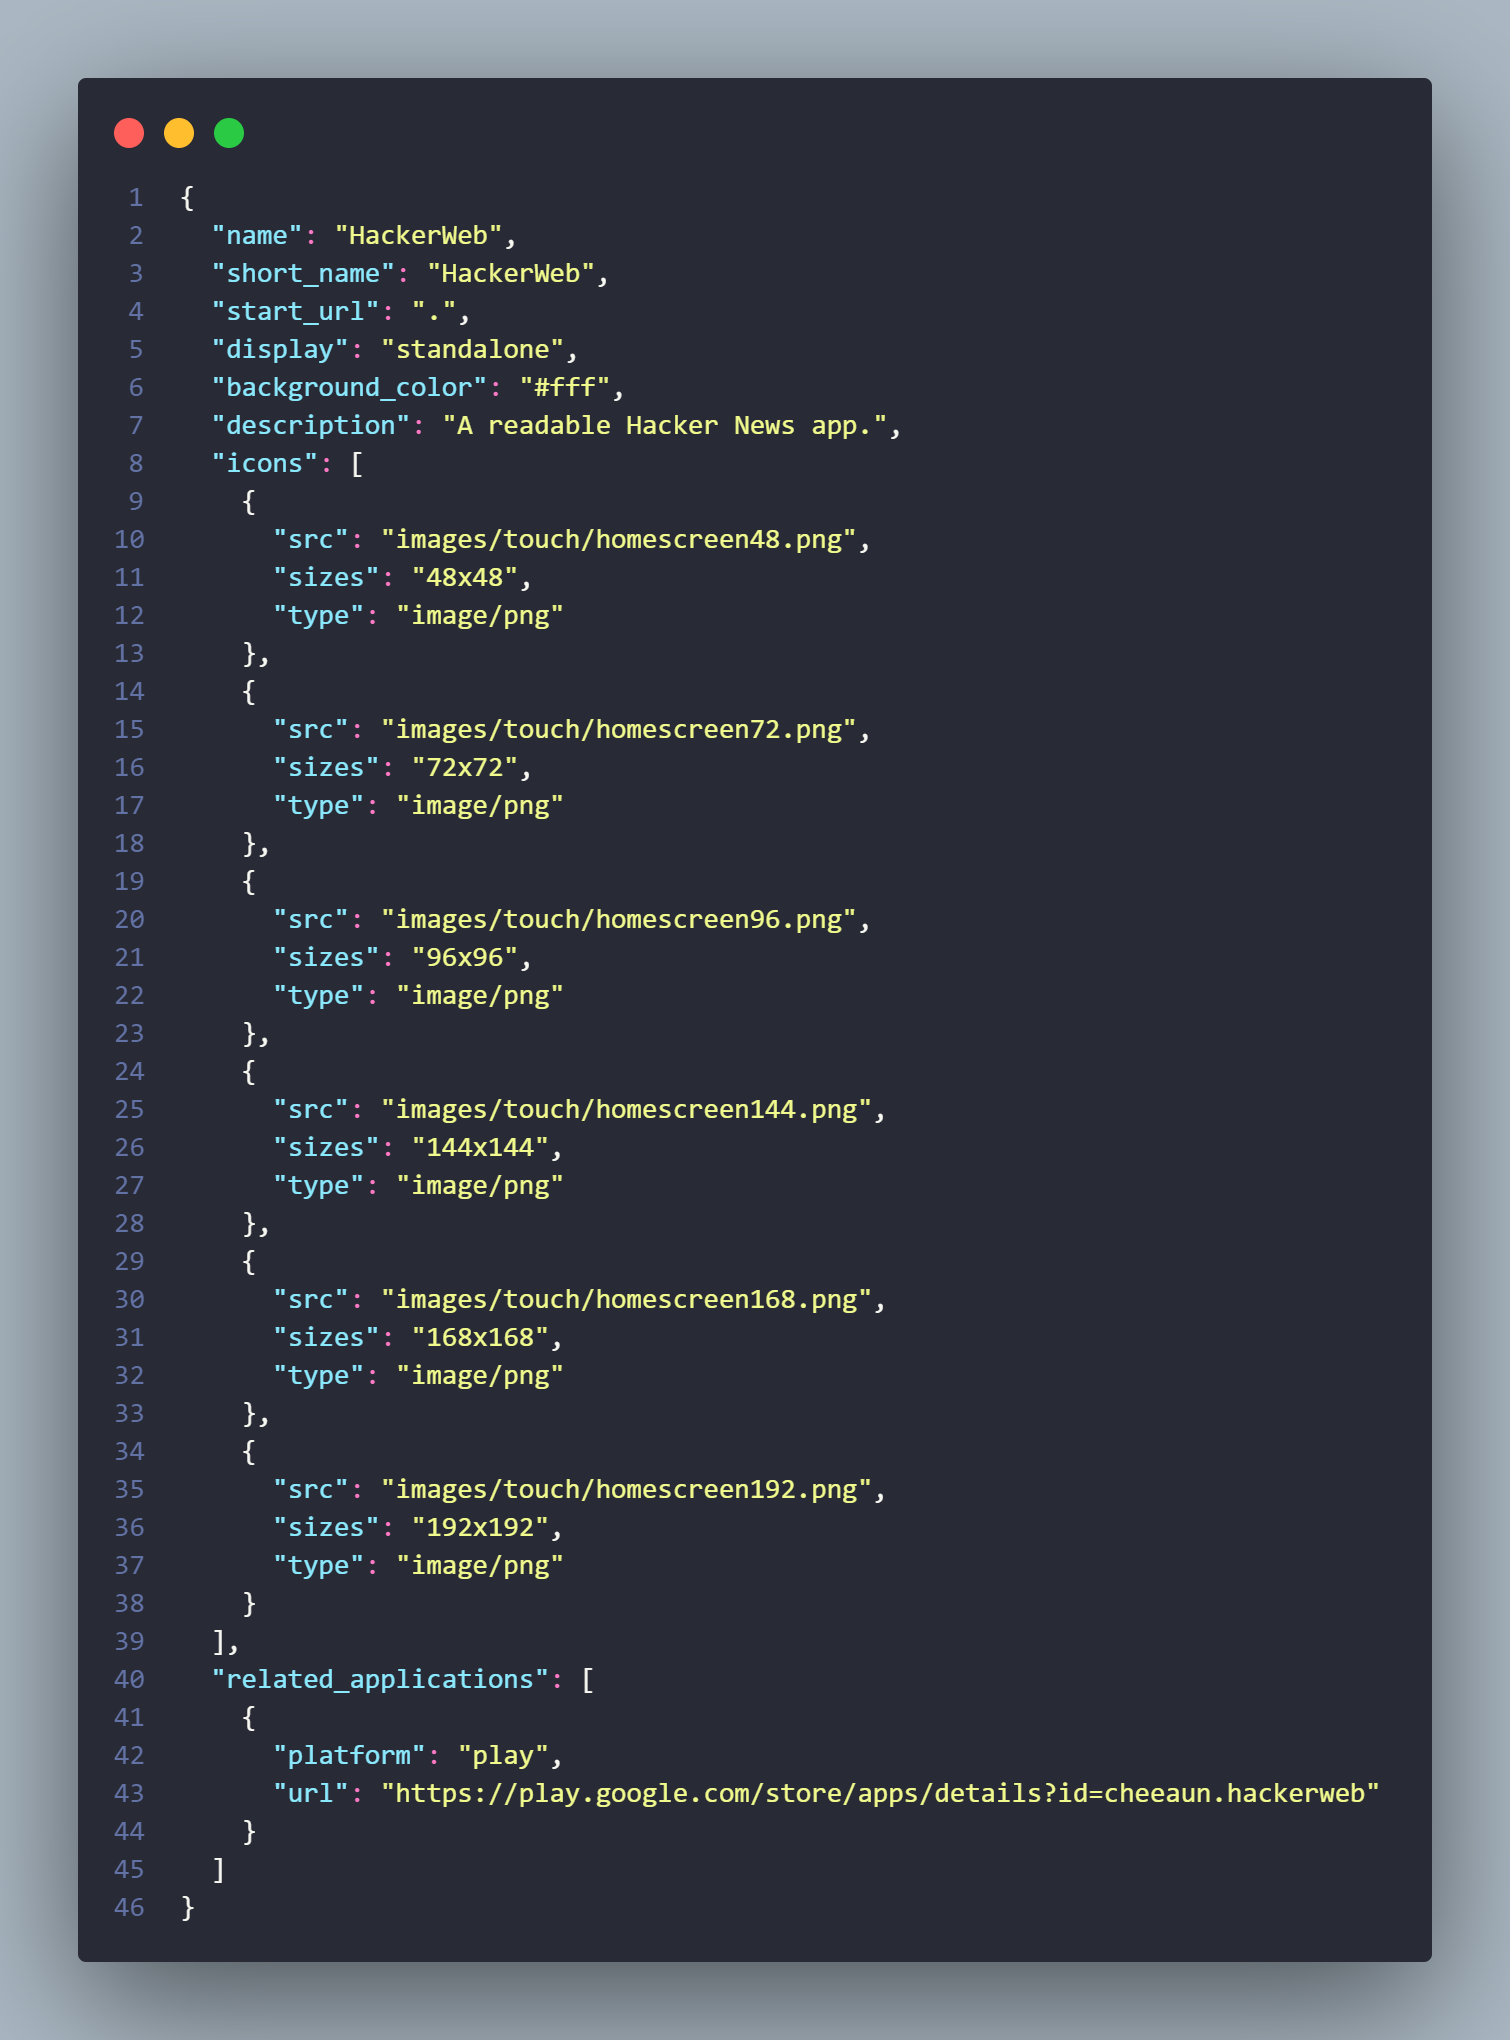
\includegraphics[width=0.7\textwidth]{img/1.png}
  \caption{Manifest example}
  \label{subd3} 
  \end{centering}
\end{figure}


\end{document}